% !TEX encoding = UTF-8 Unicode

\documentclass[11pt]{article} % use larger type; default would be 10pt

\usepackage[utf8]{inputenc} % set input encoding (not needed with XeLaTeX)
\usepackage[ngerman]{babel}
\usepackage{setspace}
\usepackage{threeparttable}
\onehalfspacing
%%% PAGE DIMENSIONS
\usepackage{geometry} % to change the page dimensions
\geometry{a4paper} % or letterpaper (US) or a5paper or\dots.
\usepackage{graphicx} % support the \includegraphics command and options
\graphicspath{ {./images/} }
%%% PACKAGES
\usepackage{booktabs} % for much better looking tables
\usepackage{array} % for better arrays (eg matrices) in maths
\usepackage{paralist} % very flexible & customisable lists (eg. enumerate/itemize, etc.)
\usepackage{verbatim} % adds environment for commenting out blocks of text & for better verbatim
\usepackage{subfig} % make it possible to include more than one captioned figure/table in a single float
% These packages are all incorporated in the memoir class to one degree or another\dots
\usepackage{amsfonts}
%%% HEADERS & FOOTERS
\usepackage{fancyhdr} % This should be set AFTER setting up the page geometry
\pagestyle{fancy} % options: empty , plain , fancy
\renewcommand{\headrulewidth}{0pt} % customise the layout\dots
\lhead{}\chead{}\rhead{}
\lfoot{}\cfoot{\thepage}\rfoot{}
\usepackage[arrow, matrix, curve]{xy}
%%% SECTION TITLE APPEARANCE
\usepackage{sectsty}
\allsectionsfont{\sffamily\mdseries\upshape} % (See the fntguide.pdf for font help)
% (This matches ConTeXt defaults)

%%% ToC (table of contents) APPEARANCE
\usepackage{amsthm}
\usepackage[nottoc,notlof,notlot]{tocbibind} % Put the bibliography in the ToC
\usepackage[titles,subfigure]{tocloft} % Alter the style of the Table of Contents
\renewcommand{\cftsecfont}{\rmfamily\mdseries\upshape}
\renewcommand{\cftsecpagefont}{\rmfamily\mdseries\upshape} % No bold!
\usepackage{oldgerm}
\usepackage{amsmath}
\usepackage{mathtools}
\usepackage{hyperref}% http://ctan.org/pkg/hyperref
\usepackage{lipsum}% http://ctan.org/pkg/lipsum
\usepackage{calc}
\usepackage{graphicx}
\allowdisplaybreaks
\newcommand{\argmin}{\operatornamewithlimits{arg\,min}}
\newcommand{\argmax}{\operatornamewithlimits{arg\,max}}
\newcommand{\sign}{\operatorname{sign}}
\newlength\mylength
\setlength\mylength{(\widthof{long long long long long}-\widthof{short})/2}
\newcommand{\NAME}{DEFINITION}
\renewcommand{\contentsname}{Inhaltsverzeichnis}
\renewcommand\refname{Literatur}
\renewcommand{\abstractname}{Zusammenfassung}

\setlength\parindent{0pt}
\begin{document}
\setcounter{tocdepth}{4}
\newtheorem{lem}{Lemma}[subsection]
\newtheorem{defi}[lem]{Definition}
\newtheorem{satz}[lem]{Satz}
\newtheorem{cor}[lem]{Korollar}
\newtheorem{theo}[lem]{Theorem}
\newtheorem{prop}[lem]{Proposition}
\newtheorem{conv}[lem]{Konvention}
\newtheorem{bsp}[lem]{Beispiel}
\newtheorem{boxh}{boxh}


Eine plausible Erklärung dafür, warum sich moderne Neuronale Netze durch winzige Änderungen im Bildsignal massiv stören lassen, und dafür dass oftmals die selbe Störung eine Vielzahl verschiedener Netze zu Klassifikationsfehlern bringen kann, liefern Goodfellow et al. in \cite{Goodfellow}: 
 Formal gesehen handelt es sich bei neuronalen Netzen um die abwechselnde Verkettung (affin) linearer Funktionen und nichtlinearer Aktivierungsfunktionen. 
Affin lineare Funktionen haben die Eigenschaft, dass die selbe Störung des Arguments unabhängig von ebendiesem Argument zur selben (absoluten) Störung des Funktionswertes führt. Ohne die nichtlinearen Aktivierungsfunktionen würde also eine Bildstörung, die für ein Bild dazu führt. dass das neuronale Netz einer Klasse einen höhere Wert zuordnet, auch bei jedem anderen Bild den ausgegebene Wert für diese Klasse erhöhen, und zwar um genau so viel. \\  \\ Qualitativ dürfte sich daran in den meisten Fällen auch durch die für Klassifikation normalerweise am Ende des neuronalen Netzes stehende Softmaxfunktion, die gegebene Werte in eine Wahrscheinlichkeitsverteilung umwandelt nichts ändern: die Softmaxfunktion nimmt das Exponential jedes Eingangswerts und normiert den resultierenden Vektor zu einer Wahrscheinlichkeitsverteilung. Aufgrund der Monotonie der Exponentialfunktion sorgt eine höhere Eingabe für ein Argument normalerweise auch für eine höhere zugehörige Wahrscheinlichkeit, auch wenn es gelegentlich durch Verschiebung der relativen Größen der anderen Eingabewerte anders kommen kann. Für weitestgehend lineare Netze erwarten wir also, dass die selbe Bildstörung für eine Vielzahl von Bildern sehr ähnliche Effekte hat. \\ \\  Moderne Neuronale Netze sind nun aber oftmals um das Training zu erleichtern genau darauf ausgelegt, sich möglichst linear zu verhalten: Bei Netzen die die Sigmoidfunktion, die sich nahe der Null quasi linear verhält und mit zunehmendem Abstand zur Null aussättigt und sich asymptotisch einer Konstanten annähert verwenden, wird meist versucht, die Eingabewerte größtenteils auf den quasi-linearen Bereich der Aktivierungsfunktion zu Beschränken um das Training zu erleichtern. Die populären ReLU-Funktionen verhalten sich stets linear oder geben Null aus. Auch wenn sich theoretisch jede stetige Funktion durch ein Netz mit ausreichend vielen ReLU-Neuronen approximieren lässt, wofür es essentiell ist, dass die ReLU-funktion eben nicht immer linear ist, ist ein Neuronales Netz, das ausschließlich ReLU-Neuronen besitzt nur in der Lage, stückweise lineare Funktionen exakt darzustellen. Die Anzahl der ''Stücke'' wächst mit der Anzahl und Größe der Schichten des Netzes aufgrund der damit verbundenen häufigeren Anwendung der Aktivierungsfunktion, weshalb sich gerade kleinere Netze mit ReLU in großen Bereichen des Eingaberaums linear verhalten. \\ Zwei Netze, die in der selben Region linear sind und die selbe Zielfunktion approximieren sollen, werden sich weiterhin in dieser Region meistens ähnlich verhalten, da die optimale Approximation einer Funktion durch lineare Funktionen für die meisten gängigen Maße für Approximationsgüte (wie zum Beispiel die $L2$-Norm) eindeutig ist. \\ \\ Die Ähnlichkeit neuronaler Netze zu linearen Funktionen erklärt nicht nur, warum Täuschungsversuche oftmals generalisieren, sondern kann auch motivieren, warum oftmals kleine Störungen ausreichen um einen großen Effekt auf die Ausgabe eines Netzes zu haben: Linearität und eine hohe Dimension des Eingaberaums erlauben, dass sich die einzeln betrachtet kleinen Effekte kleiner Störungen einzelner Dimensionen aufaddieren, was bei zufälligen Störungen kein Problem ist, da sich die Veränderungen in der Ausgabe in Erwartung aufheben, aber bei gezielten Attacken zu massiven Fehlern in der Ausgabe durch winzige Störungen in der Eingabe führen kann.  \\ \\
Unser erster und einfachster Ansatz basiert vollständig auf der angenommenen Ähnlichkeit des zu täuschenden neuronalen Netzes zu einer linearen Funktion: Ausgehend von einem Schwarzen Bild, wird für jede Quadratische Pixelgruppe auf einem Raster einzeln jeder Farbkanal separat von $0$ auf $255$ (den Maximalwert) gestellt und die Ausgabe des zu täuschenden neuronalen Netzes für das resultierende Bild gespeichert. (Ein analoger Ansatz für weißen Hintergrund ist natürlich auch möglich) Unter Annahme von Linearität lässt sich so die maximal Mögliche Störung der Ausgabe durch die Veränderung der Pixelgruppe auf diesem Kanal bestimmen. Im linearen Fall addieren sich die Effekte der Störung zudem auf, sowohl bezüglich der Farbkanäle als auch bezüglich der Pixelgruppen. Um nun das Netz dazu zu bringen, ein Bild als gegebenes Verkehrszeichen zu klassifizieren, beginnen wir mit einem Schwarzen Bild und aktivieren einen Farbkanal immer dann für eine Pixelgruppe, wenn dessen Aktivierung auf dem Schwarzen Bild zu einer Vergrößerung der Konfidenz des Netzwerkes in das gegeben Verkehrszeichen über einem Schwellenwert geführt hat. Für ein beliebiges Ausgangsbild  können wir nun das veränderte schwarze Bild als ''Sticker'' verwenden: Pixelgruppen des Ausgangsbildes, bei denen der Sticker nicht schwarz ist werden durch die Pixelgruppe auf dem Sticker ersetzt (alternativ kann das ganze auch kanalweise ''transparent'' gemacht werden). Die Linearität sorgt nun für eine ähnliche Vergrößerung der Konfidenz wie bei dem Schwarzen Bild. Da wir nicht auf allen Kanälen mit 0 starten, ist der Effekt etwas schwächer als bei dem schwarzen Ausgangsbild. Trotz der wahrscheinlich nichttrivialen Abweichung von der Linearität des Netzes lassen sich mit dieser Methode bereits gute Resultate erzielen: \\

\begin{threeparttable}
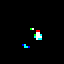
\includegraphics[height=2.8cm]{2_block25_0_010_99999928}
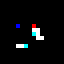
\includegraphics[height=2.8cm]{4_block25_0_010_99999976}

\includegraphics[height=2.8cm]{7_block_central0_010_98064834}
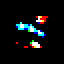
\includegraphics[height=2.8cm]{2_block3_0_011_0}
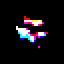
\includegraphics[height=2.8cm]{2_block4_0_010_99945539}
\begin{tablenotes}
\footnotesize 
\item\textit{ Sticker für Pixelblockgröße 7, 4 und 2 und die Klasse ''Baustelle'', sowie Sticker der Größe 2 für die Klassen ''Zulässige Höchstgeschwindigkeit 60'', sowie -''70''. Die Konfidenzen liegen für den 7-Pixel Sticker bei $98\%$ und sonst stets über $99.9\%$.
Die Gesamtgröße des Rasters betrug für den ersten Sticker $14\times14$ und für die anderen jeweils $32\times32$ Pixel. Für die Generierung der Sticker wurden für die verschiedenen Blockgrößen 30, 256 und 812 Anfragen an das neuronale Netz benötigt (Abfrage der Konfidenz für einzelne Blöcke sowie Probe ob der Sticker auf schwarzem Hintergrund zu mehr als $95\%$ Konfidenz führt). Dadurch konnten mit einem Schwellenwert von $1\%$ für die Aufnahme eines Blockes Sticker für 3, 16 und 9 verschiedene Klassen generiert werden. }
\end{tablenotes}
\end{threeparttable}
\\  

 \begin{threeparttable}
\begin{small}
\begin{tabular}{lllll}

\textbf{Konfidenz} & kein Sticker & 2-Block ($32\times 32$) & 4-Block ($32 \times 32$) & 7-Block ($14 \times 14$) \\
Geschwindigkeit 120               &  0.02013     &          0.84139                       &      0.898033                            &  0.13658  \\
Verbot der Einfahrt                &         0.13153                         &                0.64134                 &       0.73279                           &    0.63858      \\
Baustelle                   &                  0.10344                         &       0.62279                          &               0.74832                   &  0.41303
\end{tabular}
\end{small}
 \begin{tablenotes}
      \footnotesize
      \item\textit{Durchschnittliche Konfidenzen für den Stickerangriff auf drei verschiedene Klasse, jeweils evaluiert an 25 Testbildern. Mehr tatsächlich von den Stickern ausgefüllte Fläche führt zu höheren Konfidenzen. Mehr Details (kleinere Blöcke) sollten dies theoretisch auch. Hier lässt sich der gegenteilige Effekt beobachten, was wohl an dem selben verwendeten Schwellenwert für die Aufnahme einer Pixelgruppe in den Sticker liegt. Da kleinere Pixelgruppen diesen nur seltener erreichen, nehmen die 2-Block Sticker deutlich weniger Platz ein (Bei der ersten Klasse $92\%$ der Fläche des 4-Block-Stickers und für den Rest jeweils weniger als die Hälfte).}
    \end{tablenotes}
  \end{threeparttable}
\\Im Gegensatz zu den folgenden Ansätzen muss für den Stickerangriff kein eigenes Neuronales Netz trainiert werden, wodurch die resultierende Attacke deutlich einfacher und billiger zu reproduzieren und auf andere neuronale Netze auszuweiten ist. Die vergleichbar starke Störung des Ausgangsbildes sorgt zwar einerseits dafür, dass manipulierte Bilder deutlich als nicht natürlich wahrnehmbar sind, andererseits lassen sich eine Vielzahl von Ausgangsbildern ohne jeglichen Mehraufwand (wie das abfragen eines anderen neuronale Netzes) stören. Weiterhin stellt die  ''Unnatürlichkeit'' der ausgegebenen Bilder für einen potentiellen Angreifer nur dann ein Problem dar, wenn diese auch als Gefahr erkannt werden. Einige der generierten Bilder sehen aus wie Sticker, die auch plausibel aus  ästhetischen oder symbolischen Gründen an einem Ort, wie zum Beispiel dem Rückfenster eines PKWs  kleben könnten. Weiterhin führen die generierten Sticker oftmals so robust zu Fehlklassifikationen, dass das Entfernen und Addieren einzelner kleinerer Pixelgruppen den Täuschungseffekt nicht beeinflusst, was es Angreifern ermöglicht, die Sticker noch unverdächtiger aussehen zu lassen. Immerhin sollte die Verteidigung gegen diesen Angriff vergleichsweise einfach sein: Da die Effektivität der Attacke stark von der Nähe des verwendeten Netzes zur Linearität abhängt, ist zu erwarten, dass die Attacke für tiefere neuronale Netze mit vielen Neuronen pro Schicht ein deutlich kleineres Problem darstellt. Auch wenn solche Netze deutlich mehr Daten benötigen um eine Überanpassung an den Trainingsdatensatz zu verhindern und zu generalisieren, ist doch hoffentlich davon auszugehen, dass für sicherheitsrelevante Anwendungen entsprechend mächtige Modelle genutzt werden, vor allem da diese auch in Szenarien ohne einen Angreifer bessere Klassifikationen liefern dürften. \\ \\ Der nächste Angriff basiert auf der ''fast gradient sign method / FGSM''\cite{Goodfellow} beziehungsweise der Iterierten Version davon aus Kurakin et al. \cite{Kurakin}. Hier verabschieden wir uns von dem Ansatz das anzugreifende Netz als global linear zu betrachten und schwächen die Annahme zu der von lokaler Linearität ab. Die lokal beste lineare Approximation für eine Funktion an einer Stelle ist durch die Ableitung (hier Gradient bzw. Jacobimatrix) gegeben. Um nun die Konfidenz, die das neuronale Netz einem Bild bezüglich einer Klasse zuordnet zu erhöhen, bewegen wir das Bild in die ''Richtung'', in der die lineare Approximation am schnellsten ansteigt, also in Richtung des Gradienten. Ausgehend vom Bild $I$ können wir ein Netz $N$, das Bildern eine Konfidenz für eine Klasse zuordnet also durch die Störung $\widetilde{I}=I+\alpha*\nabla N(I)$ dazu bringen, eine höhere Konfidenz auszugeben. Da Bilder meistens als ganze Zahlen kodiert werden, wenden wir vor dem Schritt den Vorzeichenoperator auf den Gradienten an, um wieder ein Bild zu erhalten, also: $\widetilde{I}=I+\alpha*\sign(\nabla N(I))$. Um die Genauigkeit des Verfahrens zu verbessern benutzen wir $\alpha=1$ und iterieren ausgehend vom Startbild $I_{0}$: $I_{k+1}=I_{k}+\sign(\nabla N(I_{k}))$: Anstatt einen großen Schritt in die Anfangs richtige Richtung zu gehen, machen wir viele kleine und berechnen die neue Richtung nach jedem Schritt. Dies könnte nun wiederholt werden, bis sich die Konfidenz nicht mehr erhöht, bis eine Wunschkonfidenz erreicht ist oder einfach für eine fixe Anzahl von Schritten. Je nach Ausgangsbild kann es aber bei den ersten zwei Ansätzen dazu kommen, dass das Ursprungsbild bis zur Unkenntlichkeit verformt wird und beim letzten je nach Schrittzahl zu dem selben Problem, oder aber dazu, dass sich die Konfidenz nur suboptimal verändert, gerade bei sehr nichtlinearen Netzen, wo es passieren kann, dass viele Pixel weitestgehend mit den Iterationen oszillieren. Um die Vorteile beider Ansätze zu kombinieren, benutzen wir eine hohe Maximalzahl von Schritten, um die visuelle Ähnlichkeit zu bewahren Projizieren wir das Bild jedoch nach jedem Schritt auf eine Umgebung des Ursprungsbildes: $I_{0}$: $I_{k+1}=P_{\theta}(I_{k}+\sign(\nabla N(I_{k})))$. In unserem Fall ist $P_{\theta}$ die Projektion auf die $\theta-l_{\infty}$ Kugel um das Ursprungsbild $B_{\theta}=\{ x : \max(x_{i}-I_{0})<\theta \}$, welche hier schlichtweg durch das ''Stutzen'' von zu großen Pixelstörungen gegeben ist. Neben der Projektionen auf Kugeln anderer Normen, wie der Euklidischen Distanz sind auch komplett andere Ansätze denkbar. Zum Beispiel könnte der Angriff auf einen bestimmten Teil eines Bildes oder jeden 2. Pixel beschränkt werden. \\ \\
Da moderne neuronale Netze quasi ausschließlich über gradientenbasierte Verfahren trainiert werden, sind auf neuronale Netze ausgelegte Machine Learning Bibliotheken wie Tensorflow oder das von uns verwendete Torch darauf optimiert, Gradienten analytisch und schnell und zu berechnen. Dementsprechend lässt sich die beschriebene Attacke schnell und einfach implementieren, wenn man denn Zugriff auf die Parameter des Netzes hat. In unserem Fall ist das anzugreifende Netz jedoch eine ''Blackbox'': wir können zwar Anfragen zur Klassifikation an es senden, können jedoch keine Gradienten abfragen und haben keinerlei Einblick in die verwendete Architektur und die gelernten Parameter. Die numerische Approximation der Gradienten ist unrealistisch, da wir hier für jede Iteration $64*64*3$, also mehr als 10000 Anfragen an das Netz senden müssten. Stattdessen trainieren wir unser eigenes Netz und hoffen, dass aus den Anfangs beschriebenen Gründen Angriffe auf diese ''Whitebox'' auch auf der Blackbox erfolgreich sind. Um bei der Generalisierung nachzuhelfen trainieren wir unsere Whitebox nicht auf die Klassifikation von Verkehrszeichen, sondern auf die Regression der Ausgabe der Blackbox aus Bildern. Weiterhin prüfen wir nach der Generation eines Bildes, ob dieses die Blackbox genau so gut wie die Whitebox täuscht und trainieren die Whitebox kurz darauf, die Regression für das Ausgabebild besser durchzuführen, falls das nicht der Fall sein sollte. Anschließend versuchen wir die verbesserte Whitebox ausgehend vom letzten Ausgabebild erneut zu täuschen und wiederholen den Gesamtvorgang bis sich die Ausgaben von White- und Blackbox ausreichend ähnlich sind.   
 


\begin{threeparttable}

\includegraphics[height=2.8cm]{GI}

\includegraphics[height=2.8cm]{GI2}

\includegraphics[height=2.8cm]{GI5}

\includegraphics[height=2.8cm]{GI10}

\includegraphics[height=2.8cm]{GI20}
\\

\includegraphics[height=2.8cm]{IMG_0265}

\includegraphics[height=2.8cm]{IMG_0265_2}
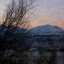
\includegraphics[height=2.8cm]{IMG_0265_5}
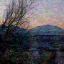
\includegraphics[height=2.8cm]{IMG_0265_10}
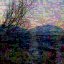
\includegraphics[height=2.8cm]{IMG_0265_20}
\begin{tablenotes}
\footnotesize 
\item\textit{Originalbild, Rauschen mit Schwellenwert 2,5,10,20. Beim Schwellenwert 2 ist quasi kein Unterschied erkennbar. Bei 5 erkennt man leichtes Rauschen. 10 rauscht stark, das Rauschen sieht aber noch natürlich aus und könnte bei Fotos auch als ISO-Rauschen wahrgenommen werden. Das Rauschen beim Schwellenwert 20 sieht bereits sehr unnatürlich aus.}
\end{tablenotes}
\end{threeparttable}
\\  

 \begin{threeparttable}
\begin{small}
\begin{tabular}{llllll}

\textbf{Konfidenz} & keine Störung & Schwelle ($\theta$) 2& Schwelle 5 & Schwelle 10 & Schwelle 20  \\
 &     0.58316         & 0.687491    &          0.80196                     &      0.88016                       &  0.93279  \\

\end{tabular}
\end{small}
 \begin{tablenotes}
      \footnotesize
      \item\textit{Durschnittliche Konfidenz für FGSM-Angriff auf 25 Testbilder und die Klasse mit der höchsten Konfidenz auf dem Originalbild für $l_{\infty}$-Schwellenwerte von 2,5,10,20. Maximale Anzahl an FGSM-Iterationen vor Korrektur der Whitebox: 25, Maximale Korrekturen: 10 Abbruch bei Blackbox-Konfidenz über $99\%$. Höhere Schwellen führen deutlich erkennbar zu mehr Konfidenz. Die hohen Werte ohne Störung sind etwas verwunderlich, obwohl der Testdatensatz zwei Verkehrsschildern sehr ähnliche Verbotsschilder enthält. }
    \end{tablenotes}
  \end{threeparttable}
  


\begin{thebibliography}{10}
\bibitem{Goodfellow} 
Goodfellow, I., Shlens, J., Szegedy, C.:
\textit{Explaining and Harnessing Adversarial Examples},
 ICLR 2015 https://arxiv.org/abs/1412.6572
 
 \bibitem{Kurakin} 
 Kurakin, A., Goodfellow, I., Bengio, S.:
 \textit{Adversarial Machine Learning at Scale},
 https://arxiv.org/pdf/1611.01236.pdf
\end{thebibliography}


 








\end{document} 
